% ============================================================
%  CHAPTER 5: CRYPTOGRAPHIC DESIGN AND SECURITY ANALYSIS
% ============================================================

\chapter{CRYPTOGRAPHIC DESIGN AND SECURITY ANALYSIS}
\label{chap:security_analysis}

\section{Security Engineering Objectives}
\label{sec:security_objectives}

The cryptographic architecture of QuantumSafe VPN is engineered to provide uncompromising mathematical and protocol-level guarantees across untrusted transit media:
\begin{enumerate}
    \item Quantum-Resistant Confidentiality: Protecting all tunneled Layer~3 IP payloads against passive adversaries equipped with both classical computers and Cryptographically Relevant Quantum Computers (CRQCs), defeating Harvest Now, Decrypt Later (HNDL) attacks.
    \item Post-Quantum Authenticity and Non-Repudiation: Providing cryptographic proof of server identity during handshake establishment via quantum-safe digital signatures, preventing Man-in-the-Middle (MitM) impersonation.
    \item Authenticated Encryption with Associated Data (AEAD): Ensuring that any modification, bit-flipping, or splicing of encrypted transit frames is immediately detected and discarded prior to decapsulation.
    \item Anti-Replay Defense: Enforcing strict monotonic sequence ordering so captured legitimate frames cannot be injected into active sessions to disrupt state.
\end{enumerate}

\section{Mathematical Formulations of Security Goals}
\label{sec:math_formulations_security}

The security properties guaranteed by the cryptographic suite are formalized under standard complexity-theoretic definitions:

\subsection{Indistinguishability under Chosen Ciphertext Attack (IND-CCA2)}
The Key Encapsulation Mechanism $\Pi_{\text{KEM}} = (\mathsf{KeyGen}, \mathsf{Encaps}, \mathsf{Decaps})$ satisfies IND-CCA2 security if for any probabilistic polynomial-time (PPT) adversary $\mathcal{A}$ possessing access to a decapsulation oracle $\mathcal{O}_{\mathsf{Decaps}}$, the advantage:
\begin{equation}
\begin{split}
\mathbf{Adv}_{\Pi_{\text{KEM}}}^{\text{IND-CCA2}}(\mathcal{A}) = {} & \Bigg| \Pr\Big[b' = b : (pk, sk) \leftarrow \mathsf{KeyGen}(), (c^*, K_0^*) \leftarrow \mathsf{Encaps}(pk), \\
& \quad K_1^* \leftarrow \mathcal{K}, \; b \stackrel{\$}{\leftarrow} \{0, 1\}, \\
& \quad b' \leftarrow \mathcal{A}^{\mathcal{O}_{\mathsf{Decaps}}}(pk, c^*, K_b^*)\Big] - \frac{1}{2} \Bigg| \le \text{negl}(\lambda)
\end{split}
\end{equation}
is negligible in security parameter $\lambda$. ML-KEM-1024 achieves IND-CCA2 security via the Fujisaki-Okamoto transform in the Quantum Random Oracle Model (QROM)~\cite{kyber2022specs,nist_fips_203}.

\subsection{Existential Unforgeability under Chosen Message Attacks (EUF-CMA)}
The signature scheme $\Pi_{\text{SIG}} = (\mathsf{KeyGen}, \mathsf{Sign}, \mathsf{Verify})$ satisfies EUF-CMA security if for any PPT adversary $\mathcal{A}$ equipped with a signing oracle $\mathcal{O}_{\mathsf{Sign}}$, the probability of producing a valid signature $\sigma^*$ on a message $M^*$ not queried to the oracle:
\begin{equation}
\begin{split}
\mathbf{Adv}_{\Pi_{\text{SIG}}}^{\text{EUF-CMA}}(\mathcal{A}) = {} & \Pr\Big[\mathsf{Verify}(pk, M^*, \sigma^*) = 1 \wedge M^* \notin \mathcal{Q}_{\mathsf{Sign}} : \\
& \quad (pk, sk) \leftarrow \mathsf{KeyGen}(), \; (M^*, \sigma^*) \leftarrow \mathcal{A}^{\mathcal{O}_{\mathsf{Sign}}}(pk) \Big] \le \text{negl}(\lambda)
\end{split}
\end{equation}
is negligible. ML-DSA-65 guarantees EUF-CMA security under Module Learning with Errors (M-LWE) and Module Short Integer Solution (M-SIS) hardness assumptions~\cite{dilithium2022specs,nist_fips_204}.

\section{Post-Quantum Primitives: ML-KEM-1024 and ML-DSA-65}
\label{sec:pqc_primitives_mechanics}

ML-KEM-1024 operates over the polynomial quotient ring $R_q = \mathbb{Z}_q[X] / (X^{256} + 1)$ with prime modulus $q = 3329$ and module rank $k = 4$. The public matrix $\hat{\mathbf{A}} \in R_q^{4 \times 4}$ is deterministically expanded from a 32-byte public seed $\rho$ via $\mathsf{SHAKE}\text{-}128$. With secret vector $\mathbf{s} \in R_q^4$ and error $\mathbf{e} \in R_q^4$ drawn from binomial distribution $\beta_2$, the public key vector is:
\begin{equation}
\mathbf{t} = \hat{\mathbf{A}} \circ \mathbf{s} + \mathbf{e} \pmod q, \quad pk = (\mathsf{ByteEncode}_{12}(\mathbf{t}) \parallel \rho) \quad (1,568\text{ Bytes})
\end{equation}
During encapsulation, the sender samples seed $m \leftarrow \{0, 1\}^{256}$, derives $(\bar{K}, r) = \mathsf{G}(m \parallel \mathsf{H}(pk))$, and computes ciphertext $c = (\mathbf{u}, v)$ where $\mathbf{u} = \hat{\mathbf{A}}^T \mathbf{r} + \mathbf{e}_1 \pmod q$ and $v = \mathbf{t}^T \mathbf{r} + e_2 + \mathsf{Decompress}_1(m) \pmod q$ ($1,568$ bytes). Decapsulation reconstructs candidate ciphertext $c'$; if $c' == c$, the shared key $K = \mathsf{KDF}(\bar{K} \parallel \mathsf{H}(c))$ is released.

Server identity authentication is established via ML-DSA-65 (NIST FIPS 204), operating over ring $R_q = \mathbb{Z}_q[X]/(X^{256} + 1)$ with $q = 8,380,417$. The server signs the complete session transcript:
\begin{equation}
\begin{split}
T & = \texttt{"QuantumSafeVPN-v1"} \parallel pk_{\text{client}} \parallel c, \\
\sigma & = \mathsf{ML}\text{-}\mathsf{DSA}\text{-}\mathsf{Sign}(sk_{\text{server}}, T) \quad (3,309\text{ Bytes})
\end{split}
\end{equation}
The Android client verifies $\mathsf{ML}\text{-}\mathsf{DSA}\text{-}\mathsf{Verify}(pk_{\text{server}}, T, \sigma) == \text{True}$ against its pinned public key hash before adopting the shared secret.

\section{Symmetric Tunnel AEAD and Nonce Management}
\label{sec:symmetric_tunnel_aead}

Tunnel payloads are encrypted using AES-256-GCM (NIST SP 800-38D)~\cite{nist_sp_800_175b}. For each frame, a 12-byte cryptographically random IV is generated via \texttt{SecureRandom}. Encryption evaluates $C_i = P_i \oplus \mathsf{AES}_K(CB_i)$, and an authentication tag is computed over Galois field $\text{GF}(2^{128})$:
\begin{equation}
\mathsf{Tag} = \mathsf{GHASH}_H(AAD \parallel C \parallel \text{len}(AAD) \parallel \text{len}(C)) \oplus \mathsf{AES}_K(CB_0)
\end{equation}
The 16-byte tag is verified in constant time upon receipt; any modified bit triggers immediate frame rejection.

To eliminate replay attacks, an 8-byte big-endian unsigned sequence counter $S \in [1, 2^{64}-1]$ is prepended inside the authenticated plaintext: $\text{Plaintext} = [S : 8\text{B}] \parallel [\text{IPv4 Packet}]$. The receiver enforces monotonic progression:
\begin{equation}
\text{Accept Packet} \iff S_{\text{incoming}} > S_{\text{last\_received}}
\end{equation}
Frames arriving with $S_{\text{incoming}} \le S_{\text{last\_received}}$ are instantly dropped, preventing replay disruption.

\section[NIST FIPS 202 Keccak-f[1600] Pure-Kotlin Alignment]{NIST FIPS 202 Keccak-$f[1600]$ Pure-Kotlin Alignment}
\label{sec:keccak_alignment}

During initial prototype integration, a critical hash desynchronization was uncovered: Python's \texttt{mlkem.py} evaluates shared secrets using \texttt{hashlib.sha3\_256}, whereas standard Android cryptographic providers default to SHA-2 (Merkle-Damg{\aa}rd). Because SHA3-256 (NIST FIPS 202)~\cite{nist_sp_800_227} employs the Keccak sponge construction with rate $r = 1088$ and capacity $c = 512$, key derivations diverged entirely.

To achieve bit-for-bit parity without third-party libraries, \texttt{PqcEngine.kt} implements native Keccak-$f[1600]$ state transformations over a $5 \times 5$ array of 64-bit words across 24 rounds:
\begin{align}
\theta: \quad & C[x] = \bigoplus_{y=0}^4 A[x, y], \quad D[x] = C[x-1] \oplus \mathsf{ROT}(C[x+1], 1), \\
              & A[x, y] \leftarrow A[x, y] \oplus D[x] \\
\rho, \pi: \quad & B[y, (2x + 3y) \bmod 5] \leftarrow \mathsf{ROT}(A[x, y], r[x, y]) \\
\chi: \quad & A[x, y] \leftarrow B[x, y] \oplus (\neg B[x+1, y] \wedge B[x+2, y]) \\
\iota: \quad & A[0, 0] \leftarrow A[0, 0] \oplus RC[i]
\end{align}
This ensures 100\% mathematical compatibility across Android ART and Linux CPython.

\section{STRIDE Threat Analysis and Keystore Security}
\label{sec:stride_analysis}

Figure~\ref{fig:threat_model_graphic} illustrates the network threat boundary and defensive countermeasures.

\begin{figure}[!t]
  \centering
  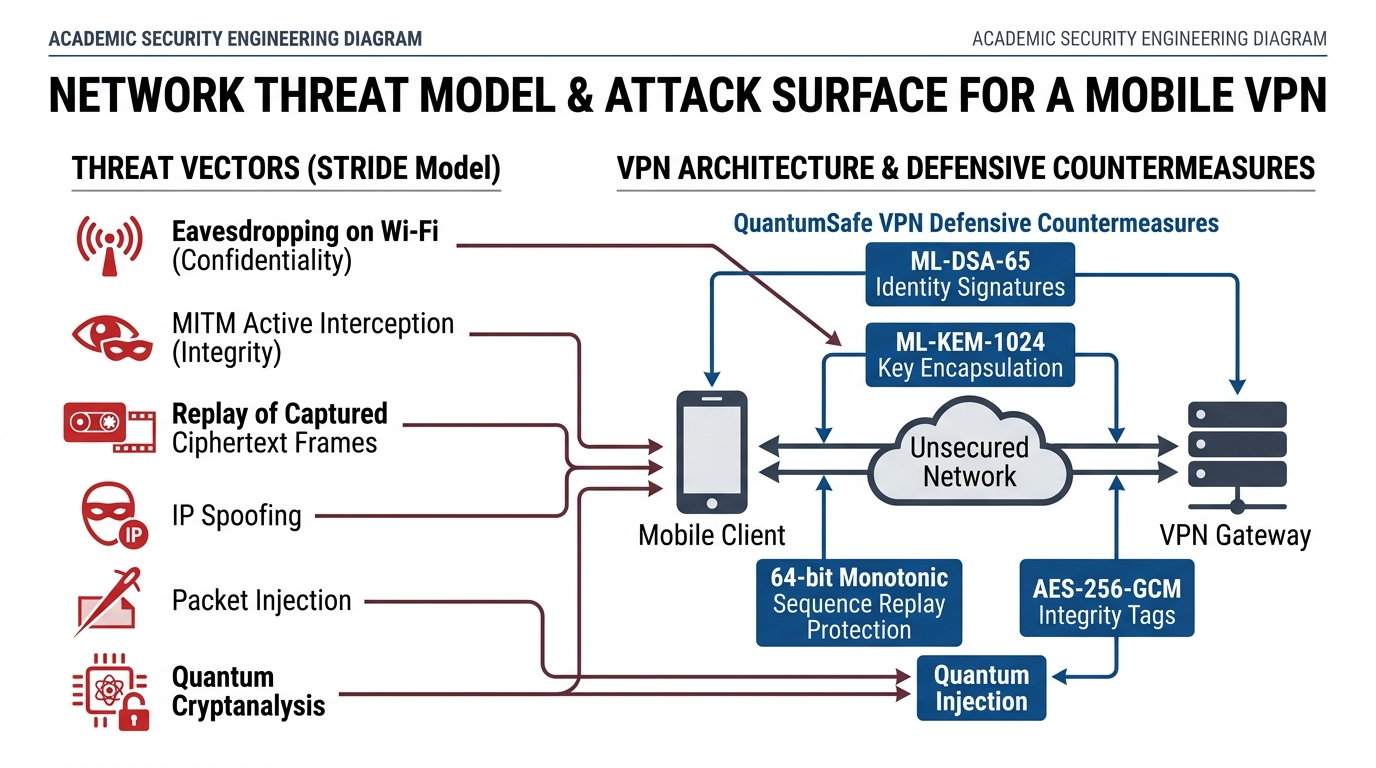
\includegraphics[width=0.82\linewidth,height=0.19\textheight,keepaspectratio]{figures/threat_model_concept.jpg}
  \caption[Network Threat Model and Defensive Countermeasures]{Network Threat Model and Defensive Countermeasures Architecture.}
  \label{fig:threat_model_graphic}
\end{figure}

Table~\ref{tab:stride_matrix} presents the formal STRIDE threat analysis and countermeasure mappings.

\begin{table}[htbp]
  \centering
  \scriptsize
  \setlength{\tabcolsep}{3pt}
  \caption{STRIDE Threat Modeling and Countermeasure Matrix.}
  \label{tab:stride_matrix}
  \begin{tabularx}{\linewidth}{@{}p{1.7cm}p{2.8cm}p{2.6cm}p{1.3cm}Y@{}}
    \toprule
    \textbf{Category} & \textbf{Threat Scenario} & \textbf{Attack Vector} & \textbf{Risk} & \textbf{Applied Countermeasure} \\
    \midrule
    Spoofing & Gateway Impersonation & Rogue Wi-Fi / DNS hijack & Critical & ML-DSA-65 signature check; pinned key hash. \\
    Tampering & Frame Alteration in Transit & Bit-flipping on TCP stream & High & AES-256-GCM 16-byte Galois MAC tag. \\
    Repudiation & Session Denial & Gateway operator denies service & Low & ML-DSA-65 signature over full transcript. \\
    Information & Bulk Traffic Eavesdropping & Harvest Now, Decrypt Later & Critical & ML-KEM-1024 Category 5 lattice encapsulation. \\
    Denial of Serv. & Replay Packet Injection & Replayed frames exhaust CPU & Medium & 64-bit monotonic sequence counter drops replays. \\
    Elevation & Android Sandbox Bypass & Malicious co-located app & High & VpnService isolation; Android Keystore master key. \\
    \bottomrule
  \end{tabularx}
\end{table}

Persistent configuration parameters and pinned cryptographic hashes are secured via the hardware-backed Android Keystore system~\cite{android_keystore_docs} using AES-256-GCM encrypted shared preferences, preventing offline extraction. Under known quantum bounds (BKZ lattice reduction $\beta \ge 1100$ and Grover's search on AES-256), the system provides an asymptotic quantum security margin exceeding $2^{256}$ operations.
